\chapter{Plasmas as Fluids}
\label{ch:Three}

\section*{Problem 3-1 (24)}
\label{sec:3-1}
We seek to use the time derivative of \(\nabla \cdot D = \nabla \cdot (\epsilon E) = 0 \) with that of \(\epsilon_0\nabla\cdot E= \sigma \), with the help of the equations \(\pp{\sigma_p}{t} -\nabla \cdot j_p = 0 \) and \(j_p = \frac{\rho}{B^2}\dd{E}{t} \) to derive the uniform low-frequency dielectic constant. We begin by substituting the fourth equation in the previous sentence into the third,
\begin{equation*}
	\pp{\sigma_p}{t} = -\nabla\cdot(\dfrac{\rho}{B^2}\dd{E}{t}).
\end{equation*}
We now apply the time derivative of the vacuum Poisson equation \(\dot{\sigma} = \epsilon_0\nabla\cdot \dot{E} \) to obtain
\begin{equation*}
	\nabla\cdot \dot{E} = -\nabla\cdot(\dfrac{\rho}{\epsilon_0B^2}\dd{E}{t}).
\end{equation*}
Rearranging the above equation gives us our desired relation
\begin{equation*}
	0 = (1 + \dfrac{\rho}{\epsilon_0B^2})\nabla \cdot E, 
\end{equation*}
where we can take \(\epsilon_R = 1 + \dfrac{\rho}{\epsilon_0B^2} = 1 + \dfrac{\mu_0\rho c^2}{B^2} \).

\section*{Problem 3-2 (25)}
\label{sec:3-2}
To begin we note that by definition of the ion cyclotron frequency and the ion plasma frequency, we say
\begin{equation*}
	\dfrac{\Omega_p^2}{\Omega_c^2} \equiv \dfrac{ne^2}{\epsilon_0m_p} = \dfrac{nm_p}{\epsilon_0B^2}.
\end{equation*}
We also say that 
\begin{equation*}
	\epsilon = \epsilon_0 + \dfrac{\rho}{B^2} \approx 1 + \dfrac{nm_p}{\epsilon_0B^2} \approx \dfrac{\Omega_p^2}{\Omega_c^2}.
\end{equation*}
We can say that the approximation holds as long as \(\epsilon \gg 1 \).

\section*{Problem 3-3 (26)}
\label{sec:3-3}
As stated in the text, equations [3-55] and [3-57] can be recovered from the divergences of equations [3-58] and [3-56], we will therefore take the divergences of these equations as follows:
\begin{equation*}
	\nabla \cdot (\nabla \times E) = \nabla \cdot \dot{B} \implies \dd{ }{t}(\nabla \cdot B) = 0,
\end{equation*}
where we have used the fact that the divergence of the curl is always zero. We therefore note that if the divergence of the magnetic field is initially zero, then it will always be zero, this is simply equation [3-57]. In order to obtain equation [3-55] we will take the divergence of equation [3-58], 
\begin{equation*}
	\nabla \cdot (n_iq_iv_i + n_eq_ev_e) = - \nabla\cdot\epsilon_0\dot{E}.
\end{equation*}
By applying the associativity of the divergence operator and the continuity equation [3-60], we obtain
\begin{align*}
	q_i(\nabla \cdot n_iv_i) + q_e(\nabla \cdot n_ev_e)=& -\nabla\cdot\epsilon_0\dot{E}\\
	q_i\pp{n_i}{t} + q_e\pp{n_e}{t}=& -\nabla\cdot\epsilon_0\dot{E}\\
	\pp{}{t}(q_in_i + q_en_e) =& -\pp{}{t}\epsilon_0\nabla\cdot E.
\end{align*}
Here we see that the final equation above implies that if the two quantities are initially equal, then they will always be equal, this is equation [3-55].
\section*{Problem 3-4 (27)}
\label{sec:3-4}
Equation [3-69] is given by
\begin{equation*}
	j_D = \left(k_BT_i + k_BT_e\right)\dfrac{B\times\nabla n}{B^2}
\end{equation*}
expressing each quantity in terms of its dimensions gives
\begin{align*}
	[j_D] =& [\text{Joule}]\dfrac{[\text{Tesla}][\text{meter}^{-4}]}{[\text{Tesla}^2]}\\
		=& \dfrac{[\text{kg}][\text{m}^2]}{[\text{s}^2]} \dfrac{[\text{kg}][\text{m}^{-4}]}{[\text{C}][\text{s}]}\\
		=& \dfrac{[\text{C}]}{[\text{m}^2][\text{s}]}.
\end{align*}
Which, are the expected units of current density.

\section*{Problem 3-5 (28)}
\label{sec:3-5}
If we take \(\Delta n = n'L \) we can say that the current \(|J_D| = |\Delta nev_y| = |n'Lev_y|\). From here, we say that if the current density is given by 
\begin{equation*}
	|j_D| = \dfrac{|J_D|}{L} = |\Delta nev_y|.
\end{equation*}
We can further say that if \(v_y \) is chosen such that the above equation agrees with equation [3-69] we can say that the dependence on \(L \) cancels and we can say that the current calculated from the particle picture will agree with a box of any width.

\section*{Problem 3-6 (29)}
\label{sec:3-6}
The expression for the electron diamagnetic drift velocity is given by
\begin{equation*}
	v_{D_e} = \dfrac{\gamma k_BT}{eB}\dfrac{\hat{z}\times\nabla n}{n}.
\end{equation*}
We can evaluate \(\nabla n \) to be
\begin{equation*}
	\nabla n = \pp{n}{x}\hat{x} = -2\dfrac{n_0}{a^2}x\hat{x}
\end{equation*}
These can be combined to yield the final equation
\begin{equation*}
	v_{D_e} = \dfrac{k_BT_e}{eB}\dfrac{2x}{a^2}\left(1 - \dfrac{x^2}{a^2}\right)^{-1}\hat{y}
\end{equation*}
The density profile over \(x \in (-a,a) \) is a quadratic with zeros at \(x=-a\) and \(x=a\), the maximum occurs at \(x=0\) and takes a value of \(n_0\); the diamagnetic drift velocity is upwards on the positive side of the plane and negative on the right side of the plane. 

If we evaluate \(v_{D_e}\) at \(x = a/2\) we obtain \(v_{D_e} = 333 \)m/s.

\section*{Problem 3-7 (30)}
\label{sec:3-7}
In order to determine the \(E\times B, v_E \) drift and the diamagnetic drift \(v_{D_e}\) we will first need an expression for the electric field, which we will obtain using \(E = -\nabla \phi \), we can express \(\phi\) using the density expressions
\begin{equation*}
	n = n_0\exp\left(\frac{-r^2}{r_0^2} \right) = n_0\exp\left(\frac{e\phi}{k_BT_e} \right) \implies \phi = \dfrac{k_BT}{e}\log\left(\dfrac{n}{n_0}\right) = \dfrac{k_BT}{e}\log\left(\dfrac{-r^2}{r^2_0}\right).
\end{equation*}
We further note that
\begin{equation*}
	\dfrac{n'}{n} = \pp{}{r}(\log\left(n\right)) = \pp{}{r}\dfrac{-r^2}{r_0^2} = \dfrac{-2r}{r^2_0}.
\end{equation*}
We will use our expression for \(\phi\) along with the fact that \(E = -\nabla \phi \) to obtain
\begin{equation*}
	E = \pp{\phi}{r}\hat{r} = \dfrac{k_BT_e}{e}\log\left(\dfrac{2r}{r_0^2}\right).
\end{equation*}
We obtain an expression for our \(E\times B\) drift by noting that since \(B\) is uniform we have
\begin{equation*}
	v_E = \dfrac{E\times B}{B^2} = -\hat{\theta}\dfrac{E_r}{B_z} = -\dfrac{k_BT_e}{eB}\dfrac{2r}{r^2_0} \hat{\theta}.
\end{equation*}
Likewise, for the diamagnetic drift, we obtain
\begin{align*}
	v_{D_e} =& -\dfrac{k_BT_e}{eB}\dfrac{n'}{n}\hat{\theta}\\
	=& -\dfrac{k_BT_e}{eB}\dfrac{-2r}{r_0^2}\hat{\theta}\\
	=& -v_E,
\end{align*}
which shows that the two drifts are indeed equal and opposite. Furthermore, we can see that the plasma rotates as a solid body by noting that since our drift velocities are in the \(\hat{\theta} \) direction and directly proportional to \(r\), we note that \(\omega \propto v_\theta/r \) and say that the rotation frequency is constant.

We note that 
\begin{equation*}
	v = v_\phi + v_E = \frac{1}{2}v_{D_e} + (-v_{D_e}) = \frac{1}{2}v_{D_e}
\end{equation*}
A sketch of the relative magnitudes of velocities from the laboratory frame of reference are shown in the figure below
\begin{figure}[!h]
	\centering
	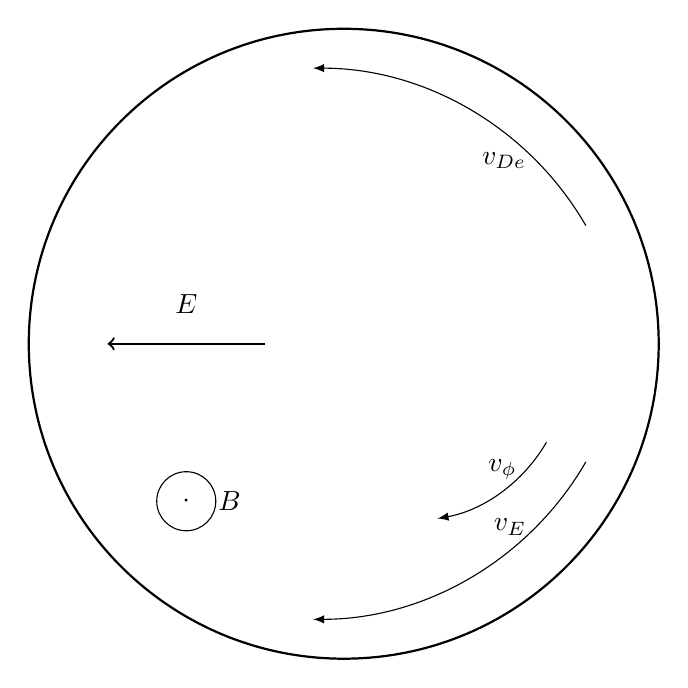
\begin{tikzpicture}
		\draw[thick] (0,0) circle (4cm);
		\draw[-latex] (3.075,1.5) arc (30:90:4cm) node[near start,left] {\(v_{De}\)};
		\draw[-latex] (3.075,-1.5) arc (-30:-90:4cm)  node[near start,left] {\(v_{E}\)};
		\draw[-latex] (2.575,-1.25) arc (-30:-80:2cm)  node[near start,left] {\(v_{\phi}\)};
		\node at (-2,-2) [circle,draw,inner sep=0pt,minimum width=0.75cm] {\(\cdot \)};
		\node at (-1.45,-2) {\(B \)};
		\draw[->, thick] (-1,0) -- (-3,0);
		\node at (-2,0.5) {\(E\)};
	\end{tikzpicture}
	\caption{Relative magnitudes and directions of \(\bm{v}_E\), \(\bm{v}_{De}\), and \(\bm{v}_\phi\)}
	\label{fig:3-7}
\end{figure}

\section*{Problem 3-8 (31)}
\label{sec:3-8}
For this problem we can simply note that 
\begin{equation*}
	j_D = ne\left(v_{D_i} - v_{D_e}\right) = \dfrac{n_0(k_BT_i + k_BT_e)}{B}\dfrac{2r}{r^2_0}\exp\left(-\dfrac{r^2}{r^2_0} \right) = 0.147 \text{A/m}^2.
\end{equation*}
In the lab frame, this current is carried entirely by ions, since \(v_e = v_E + v_{D_e} = v_E - v_E = 0 \).




